
%Transverse enhancement is included as a parametrization affecting the $Q^{2}_{QE}$  dependence in our analysis, however it is thought to be due to underlying multinucleon dynamical processes [49- 54].   Such processes are not included in
%The experiment�s simulation;  if present they could effect our measurements of vertex energy and of recoil energy in ways which are not accounted for. 

Transverse enhancement is included as a parametrization affecting the $Q^{2}_{QE}$ dependence in our analysis but is thought to be due to underlying
 multinucleon dynamical processes~\cite{Donnelly:1999sw,Carlson:2001mp,Maieron:2009an,Martini:2009uj,Amaro:2010sd,Martini:2010ex,Nieves:2013fr}. Such processes could have an 
effect on the vertex and recoil energy distributions that we do not simulate. 
Motivated by these concerns and by discrepancies observed 
in our analysis of $\nu_\mu$ quasi-elastic scattering~\cite{nuprl}, 
we have also studied the vertex energy to test the simulation 
of the number of low energy charged particles emitted in 
quasi-elastic interactions. Figure~\ref{fig:vtx_eng} shows this 
energy compared to the simulation.   A fit which modifies the
distributions to incorporate energy due to additional protons is not able 
to achieve better agreement. This might be explained if the dominant multibody 
process is $\bar{\nu}_\mu (n p) \to \mu^{+} n n$~\cite{Donnelly:1999sw,Martini:2009uj,Subedi:2008zz} 
since \minerva is not very sensitive to low energy neutrons. 
A similar analysis on neutrino mode data is consistent with 
additional protons in the final state~\cite{nuprl}.
%and is helpful 
%in drawing further conclusions about the effect of the nucleus on 
%quasi-elastic reactions

%We have done a similar analysis on neutrino mode data which is helpful  in drawing further conclusions about the effect of the nucleus on  quasi-elastic reactions~\cite{nuprl}.


\begin{figure}[tp]
\centering
%\includegraphics[width=0.45\columnwidth]{figures/vtxe_lowq2}
%\includegraphics[width=0.45\columnwidth]{figures/vtxe_highq2}
\ifnum\PRLsupp=0
  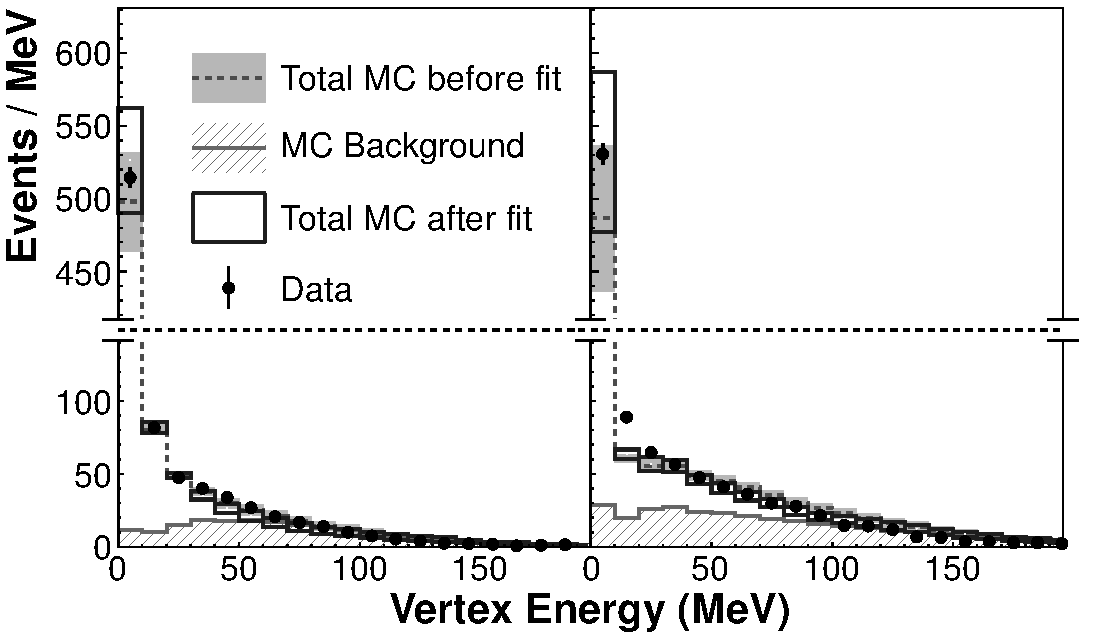
\includegraphics[width=\columnwidth]{figures/nubar_vtxE_sharedaxis_horiz}
\else
  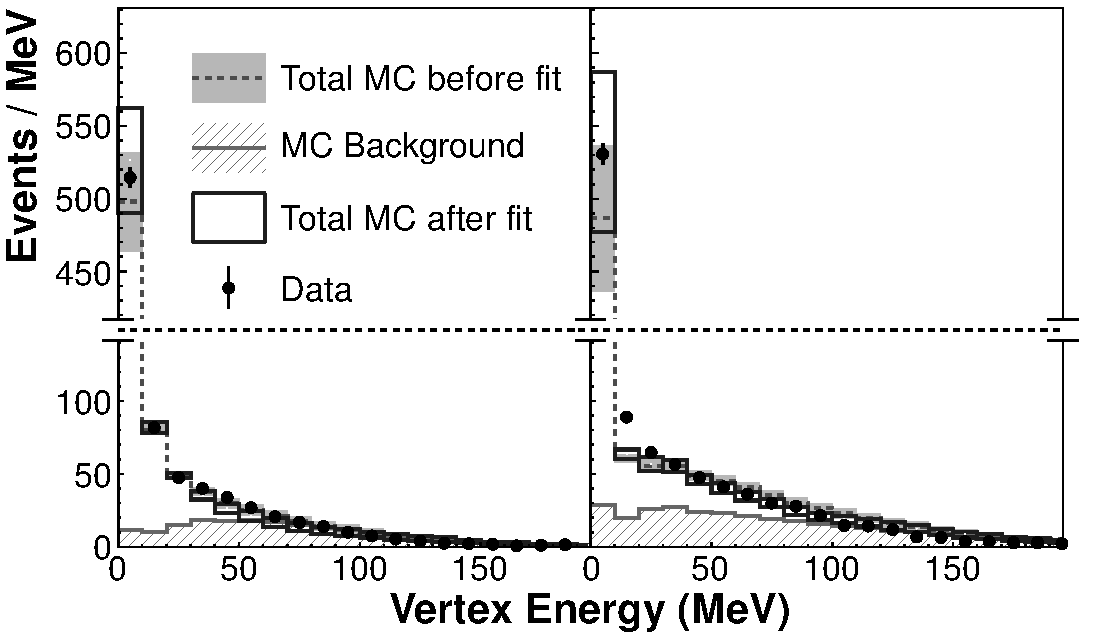
\includegraphics[width=0.7\columnwidth]{figures/nubar_vtxE_sharedaxis_horiz}
\fi
\caption{Reconstructed vertex energy of events passing the selection criteria compared to the GENIE RFG model for $Q^2_{QE} < 0.2$ GeV$^2/$c$^2$ (left) and for $Q^2_{QE} > 0.2$ GeV$^2/$c$^2$ (right).}
    \vspace{-10pt}
\label{fig:vtx_eng}
\end{figure}
